\chapter{Cibles de fonctionnement}

\section{Processus Retour d'exéprience}

\begin{figure}[h!]
	\centering
	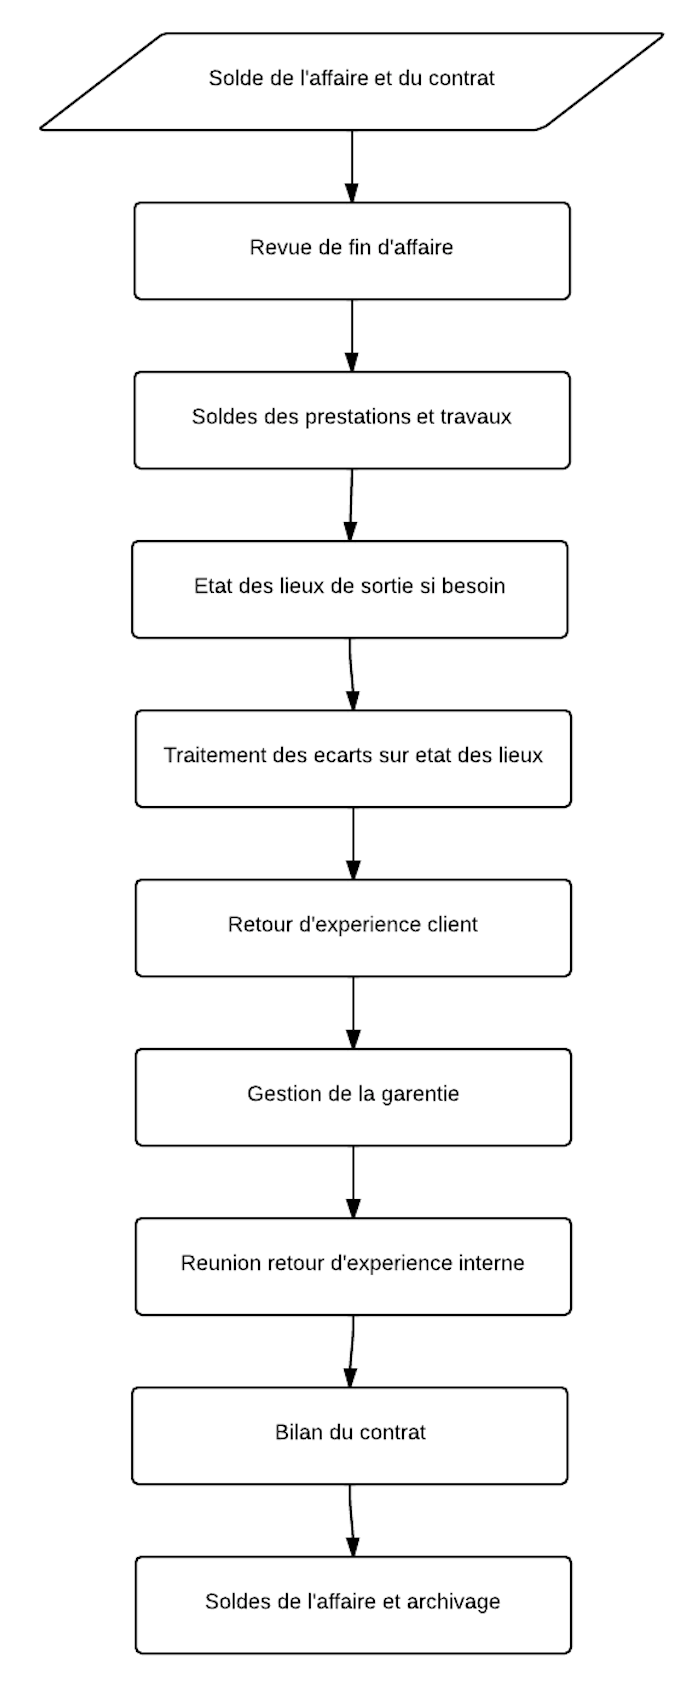
\includegraphics[width=0.45\linewidth]{images/processus_retour_experience.png}
	\caption{Processus de retour d'experience}
	\label{fig:processusRetourExperience}
\end{figure}

Ainsi l'ajout du processus \textit{retour d'\'exp\'erience client} dans le sous-processus \textit{solde
de l'affaire et du contrat} r\'epond aux exigences de SPIE Sud Est suivante~:

\begin{itemize}
    \item Base de connaissance m\'etier type de contrat~;
    \item Identification des risques techniques/financiers/organisationnels.
\end{itemize}

